\documentclass[11pt]{article}  
\usepackage[margin=1in]{geometry}
\parindent=0in
\parskip=8pt
\usepackage{fancyhdr,amssymb,amsmath, graphicx, listings,float,subfig,enumerate,epstopdf,color,multirow,setspace,bm,textcomp}
\usepackage[usenames,dvipsnames]{xcolor}
\usepackage{hyperref}
\usepackage{graphicx}
\graphicspath{{./Images}}

\pagestyle{fancy}


\begin{document} 

\lhead{Assignment \# 2}
\chead{Robert Denim Horton}
\rhead{\today}

\begin{center}\begin{Large}
CS 4720/5720 Design and Analysis of Algorithms

Homework \#2

Student: (Robert Denim Horton)
\end{Large}
\end{center}


\section*{Answers to homework problems:}
\textcolor{gray}{
For the purpose of this chapter and the following questions we will define and use the \textit{Strong Triadic Closure Assumption}.  The Strong Triadic Closure Assumption comes from chapter three where it states that for some node that has \textit{strong} connections with two other nodes, then eventually over time we assume that those two nodes will eventually share a separate and more direct connection with each other, whether the connection between the two nodes will be either \textit{weak} or \textit{strong}.\\\\
}
\begin{enumerate}
\setcounter{enumi}{1}
% Question 2
\item Consider the graph in Figure 3.21, in which each edge - except the edge connecting $b$ and $c$ - is labeled as a strong tie (S) or a weak tie (W).\\
\begin{center}
	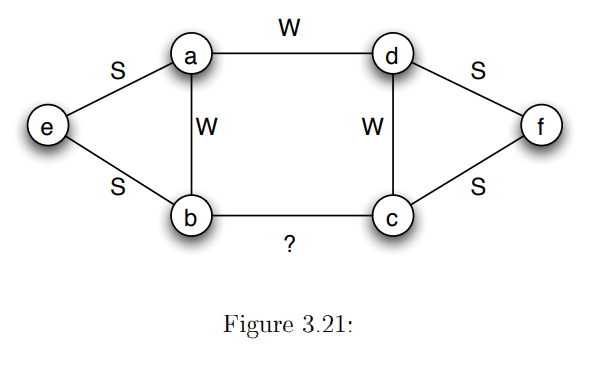
\includegraphics[scale=0.6]{Figure_3_21}
\end{center}
According to the theory of strong and weak ties, with the strong triadic closure assumption, how would you expect the edge connecting b and c to be labeled? Give a brief (1-3 sentence) explanation for your answer.\\\\
\textcolor{gray}{
With this formally defined assumption we can begin to show how to assume the strength of the edge between $b$ and $c$.  First off, it can be noticed that $c$ has one strong edge between it and $f$. We can also say the same for node $b$ and $e$.  Since we know that there is an existing edge between $b$ and $c$ and that the edge between $c$ and $f$ and $b$ and $e$, then if the edge between $b$ and $c$ was strong then there would have to be a existing edge (weak or strong) between $f$ and $b$ as well as an edge between $c$ and $e$\\
\begin{center}
	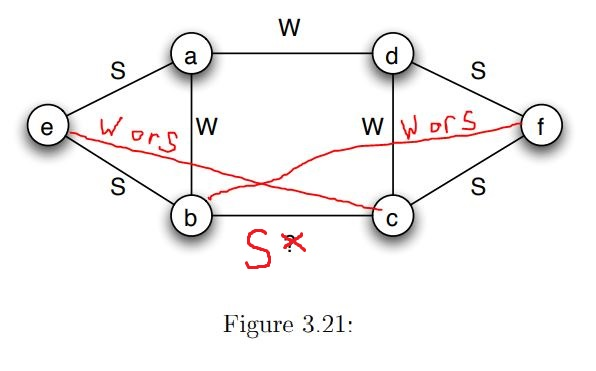
\includegraphics[scale=0.6]{Figure_3_21_Answer}
\end{center}
Therefore the edge between $b$ and $c$ is a weak connection.\\
}
% Question 3
\item  In the social network depicted in Figure 3.22, with each edge labeled as either a strong or weak tie, which nodes satisfy the Strong Triadic Closure Property from Chapter 3, and which do not? Provide an explanation for your answer
\begin{center}
	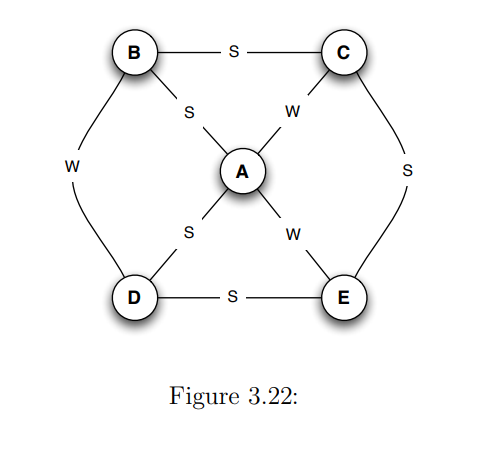
\includegraphics[scale=0.6]{Figure_3_22}
\end{center}
\textcolor{gray}{
Steeping through each node, we first evaluate node $a$ which shares connections with $b$, $c$, $d$, and $e$.  However, the only strong connections it shares are with nodes $b$ and $d$ which to share an edge.  Evaluating the next node $b$, we see it is connected to nodes $a$, $c$, and $d$.  The only pair of nodes that is shares a strong connection with is node $a$ and $c$ which do share an edge with each other. Node $c$ shares connections with $a$, $b$, and $e$.  The only strong connections $c$ has are with node $e$ and $b$ which are not directly connected by an edge, so this node violates the Strong Triadic Closure property. next we look as node $d$, which like $c$ is connected to the same nodes but has strong connections to $a$ and $e$ which validates the Strong Triadic Closure property. Lastly, node $e$ if evaluated which like $b$ has connections to $a$, $c$, and $d$.  Here we see that $e$ has two strong connections between $d$ and $c$ but $d$ and $c$ don't share a direct connection together and therefore violated the Strong Triadic Closure property.\\
\begin{center}
	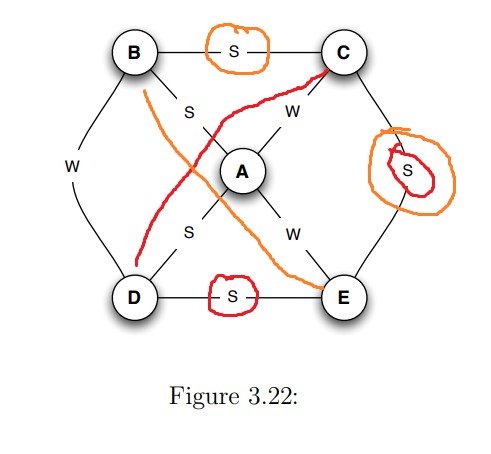
\includegraphics[scale=0.6]{Figure_3_22_Answer}
\end{center}
Hence, $A$, $B$, \& $D$ satisfy the Strong Triadic Closure property where $C$ \& $D$ do not.\\
}
% Question 4
\item In the social network depicted in Figure 3.23 with each edge labeled as either a strong or weak tie, which two nodes violate the Strong Triadic Closure Property? Provide an explanation for your answer
\begin{center}
	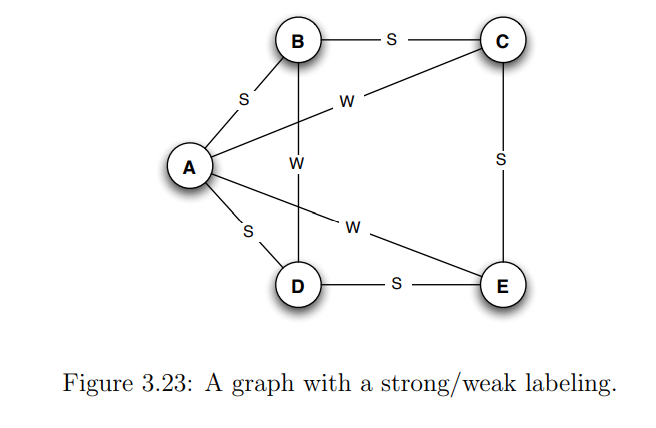
\includegraphics[scale=0.6]{Figure_3_23}
\end{center}
\textcolor{gray}{
Proceeding as we did in question 3, we simply walk through each node and look at the pairs it has and make sure that if any pair of strong edges are connected to that node that the nodes the edges are connected to posses either a strong ro weak connection.  Starting with edge $a$ we can see that for the two strong connection it posses that the coresponding nodes are connected by a weak edge.  Next, node $b$ seems to posses strong connections with $a$ and $c$ with holds true for the Strong Triadic Closure property.  As for node $c$ we see two strong connections between node $b$ and node $e$ which violates the Strong Triadic property. Same can be said for node $e$ which appears to have two strong connections, one bwteen $d$ and $c$ which do not have a strong or weak connection between them also violating the Strong Triadic Closure property.  Lastly we see that the only pair of nodes that node $d$ shares strong connections with do posses a weak connection them, node $e$ and $a$.\\
\begin{center}
	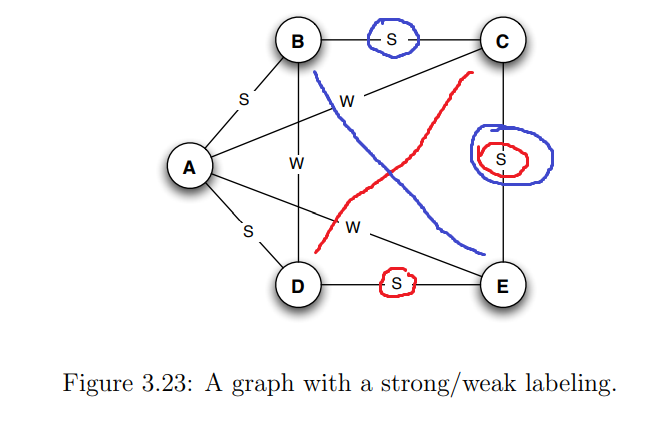
\includegraphics[scale=0.6]{Figure_3_24_Answer}
\end{center}
Thus, $C$, \& $E$ violate the Strong Triadic Closure property.\\
}
% Question 5
\item  In the social network depicted in Figure 3.24, with each edge labeled as either a strong or weak tie, which nodes satisfy the Strong Triadic Closure Property from Chapter 3, and which do not? Provide an explanation for your answer.
\begin{center}
	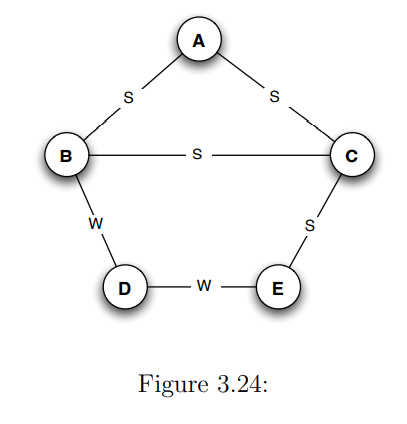
\includegraphics[scale=0.6]{Figure_3_24}
\end{center}
\textcolor{gray}{
Once again we proceed as we did in questions 3 \& 4, we walk through each nodes and evaluate each pair of nodes that nodes posses. As we can see node $a$, $b$, and $c$ all share strong connections with each making node $a$ satisfy the Strong Triadic Closure property.  looking at the rest of the nodes it is pretty easy to see that the only node left with two strong edges that aren't shared with node $a$ is node $c$.  Node $c$ shares strong connections between nodes $b$ and $e$ which do not share a connection of any strnegth and violates the STrong Triadic Closure property. \\
\begin{center}
	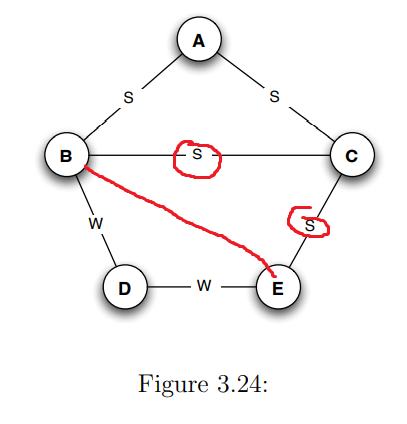
\includegraphics[scale=0.6]{Figure_3_25_Answer}
\end{center}
Thus, $c$ is the only node that does not satisfy the Strong Triadic Closure property.\\
}
\end{enumerate}
\end{document}
